\documentclass{diploma}


% makes pdf searchable & copyable
% \usepackage{cmap}

% input encoding
% \usepackage[utf8]{inputenc}

% font encoding
% \usepackage[T2A]{fontenc}

% add languages support
% \usepackage[ukrainian,english]{babel}

\begin{document}
% \maketitlepage{Борисенко Павло Борисович}{КМ-02}{ст. викл. Любашенко Н.Д.}{доцент, к. ф.-м. н. Шубенкова І.А.}{Система паралельного пошуку}

% \assigment{
    % StudentName={Борисенку Павлу Борисовичу},
    % ThesisName={\invcommas{Моделювання процесів конвекції-дифузії з переважанням дифузії}},
    % AdvisorName={ст. викладач Любашенко Наталія Дмитрівна},
    % Order={\invcommas{28}~травня~2014~р.~\No~995-C},
    % ApplicationDate={\invcommas{15}~червня~2014~р.},
    % InputData={\begin{itemize}
            % \item алгоритм методу граничних елементів;
            % \item дані задачі дифузії.
        % \end{itemize}},
    % Contents={\begin{itemize}
            % \item аналіз існуючих методів вирішення задачі;
            % \item вибір омтимального методу;
            % \item програмна реалізація;
            % \item порівняння результатів.
        % \end{itemize}},
    % Graphics={\begin{itemize}
            % \item блок-схеми алгоритмів;
            % \item знімки екранних форм.
        % \end{itemize}},
    % AssigmentDate={\invcommas{01}~жовтня~2013~р.},
    % Calendar={& & & \\},
    % StudentPIB={Борисенко П.Б.},
    % AdvisorPIB={Любашенко Н.Д.}
% }

% set one and half spacing size
% \usepackage{setspace}
% \onehalfspacing
% \renewcommand{\baselinestretch}{1.4}

% indent first paragraph
% \usepackage{indentfirst}

% for math symbols
% \usepackage{amsmath}
% \usepackage{amssymb}

% so tables will stay in place
% \usepackage{float}
% \restylefloat{table}

% include pictures
% \usepackage[pdftex]{graphicx}

% change the settings of counters
% \usepackage{chngcntr}

% change sections formating
% \usepackage{titlesec}
% \titleformat*{\section}{\normalfont \bfseries \center}
% \titleformat*{\subsection}{\normalfont \bfseries}
% \titleformat*{\subsubsection}{\normalfont \bfseries \itshape}
% add dot to the end of numbering
% \titlelabel{\thetitle. }

% write pseudocode examples
% \usepackage{algpseudocode}

% \usepackage{etoolbox}
% \newfontfamily{\codefont}{Menlo}
% \AtBeginEnvironment{algorithmic}{\codefont}

% add option to all lists
% \usepackage{enumitem}
% \setitemize{parsep=0pt}
% \renewcommand{\labelitemi}{--}

% specify page spacing
% \usepackage[top=2cm, bottom=2cm, left=3cm, right=2cm]{geometry}
% some more margins and indents
% \setlength{\evensidemargin}{0.5cm}
% \setlength{\oddsidemargin}{0.5cm}
% \setlength{\textheight}{25cm}
% \setlength{\textwidth}{16cm}
% \setlength{\parindent}{1cm}

% specify font
% \renewcommand{\familydefault}{\rmdefault}

% reformat table and figure numbering
% \renewcommand{\thetable}{\thesection .\arabic{table}}
% \renewcommand{\thefigure}{\thesection .\arabic{figure}}

% don't display subsubsection in TOC
% \setcounter{tocdepth}{2}
% \pagestyle{plain}
% \pagenumbering{arabic}

	\selectlanguage{ukrainian}

    \maketitlepage{Крамаренко Олексій Андрійович}{КП-01}
        {ст. викл. Любашенко Н.Д.}{доцент, к. ф.-м. н. Шубенкова І.А.}
        {Система паралельного пошуку у структурах даних гри Го}
        {асистент Онай М.В. }

    \assigment{
        StudentName={Борисенку Павлу Борисовичу},
        ThesisName={\invcommas{Моделювання процесів конвекції-дифузії з переважанням дифузії}},
        AdvisorName={ст. викладач Любашенко Наталія Дмитрівна},
        Order={\invcommas{28}~травня~2014~р.~\No~995-C},
        ApplicationDate={\invcommas{15}~червня~2014~р.},
        InputData={\begin{itemize}
                \item алгоритм методу граничних елементів;
                \item дані задачі дифузії.
            \end{itemize}},
        Contents={\begin{itemize}
                \item аналіз існуючих методів вирішення задачі;
                \item вибір омтимального методу;
                \item програмна реалізація;
                \item порівняння результатів.
            \end{itemize}},
        Graphics={\begin{itemize}
                \item блок-схеми алгоритмів;
                \item знімки екранних форм.
            \end{itemize}},
        AssigmentDate={\invcommas{01}~жовтня~2013~р.},
        Calendar={& & & \\},
        StudentPIB={Борисенко П.Б.},
        AdvisorPIB={Любашенко Н.Д.}
    }

    \annotation{Анотація}
Дипломна робота присвячена розробці математичних та програмних засобів для моделювання процесів конвекції-дифузії з переважанням дифузії.

У рамках роботи проведено аналіз підходів до математичного моделювання процесів конвекції-дифузії, що виникають в прикладних задачах фізики твердого тіла, гідро- та аеродинаміки, біологічних та медичних дослідженнях. Обрано математичну модель задачі з урахуванням переважання дифузних процесів.

Розглянуто способи чисельного моделювання процесів конвекції-дифузії з переважанням дифузії на основі обраної математичної моделі та обгрунтовано використання методу граничних елементів.

Розроблено програмне забезпечення, що реалізовує обрані методи моделювання дифузних процесів.

Ключові слова: процес конвекції-дифузії, дифузія, метод граничних елементів, метод колокації.

\annotation{Abstract}
In this thesis we consider the development of mathematical and software tools for simulation of convection-diffusion processes with diffusion prevalence.

In this paper we perform the analysis of theorethical approaches to convection-diffusion simulation that can be applied to the different problems in solid state physics, hydrodynamics, aerodynamics, biology and medical studies. We choose the mathematical model of this problem subject to prevalence of diffusion.

We discuss the methods of numerical modeling of convection-diffusion processes with diffusion prevalence based on choosed mathematical model and substantiate using of boundary elements method.

We describe software tools for simulation of diffusion processes developed as part of this thesis.

Keywords: convection-diffusion process, diffusion, boundary elements method, collocation method.

\annotation{Аннотация}
Дипломная работа посвящена разработке математических и программных средств для моделирования процессов конвекции-диффузии с преобладанием диффузии.

В рамках работы проведено анализ подходов к математическому моделированию процессов конвекции-диффузии, которые возникают в прикладных задачах физики твердого тела, гидро- и аеродинамики, биологических и медициских исследованиях. Выбрано матматическую модель задачи с учетом преобладания диффузных процессов.

Рассмотрено способы численного моделирования процессов конвекции-диффузии с преобладанием диффузии на основании выбраной математической модели и обосновано использование метода граничных элементов.

Разработано програмное обеспечение, реализующее выбраный метод моделирования диффузных процессов.

Ключевые слова: процесс конвекции-диффузии, диффузия, метод граничных элементов, метод коллокации.


    \tableofcontents


	\newpage
\section{Вступ}
\addcontentsline{toc}{section}{Вступ}
Го --- стародавня китайська стратегічна гра на двох гравців.
Вона є антагоністичною\footnote{Антагоністичні ігри —-- ігри з двома гравцями які мають прямо протилежні інтереси} грою з повною інформацією\footnote{Гра з повною інформацією --- термін теорії ігор, що позначає логічну гру, в якій для суперників відсутній елемент невизначеності}.
В го грають два гравці --- ``Чорні'' та ``Білі''. Вони по черзі розміщують на дошці, що складається з перетину 19 на 19 ліній, камені свого кольору.
Го територіальна гра, тобто гравець, що під кінець гри має більшу територію --- виграє.
Як і для багатьох інших подібних ігор, були спроби створити комп'ютерні програми, що гарно грають в го, але це виявилося справжнім викликом для програмістів.
Складність обчислення партій в го на кілька порядків більша за шахи.
На кожному кроці можливі близько 200—300 ходів, статична ж оцінка життя груп каменів фактично неможлива.
Одним ходом тут можна цілком зіпсувати всю гру, навіть коли решта ходів були дуже добрі.
Тому програми для гри в го не використовують таких алгоритмів, як шахові програми, а замість того зазвичай мають кілька десятків модулів для оцінки різних аспектів гри і під час аналізу намагаються використовувати ті ж самі поняттями, що й люди.
Попри це вони і далі грають дуже слабко та програють навіть не дуже сильним аматорам.

Перша програма для гри в Го була написана Альбертом Зобріст в 1968 році як частина дисертації по розпізнаванню образів. Він використав функцію впливу для оцінкі території і Зобріст-хешування для виявлення ситуацій Ко.

Останні розробки в пошуку Монте-Карло по деревах і машинному навчанню принесли кращі результати для програм, що грають в го на маленькій дошці 9x9. У 2009 році з'явилися перші подібні програми, що могли змагатися з низькими данами на дошках розміром 19х19.

Усі програми, що грають в го повинні оперувати деякими структурами даних (наприклад такими, що репрезентують поточний стан дошки або гри).
Більшість з таких програм засновані на створенні великої кількості різних партій, та подальшому їх аналізі.
Саме тому питання пошуку у подібних структурах даних дуже актуальне, адже його оптимізація корінним чином вплине на роботу та якість програм, що грають в го.

	\newpage
\section{Аналіз існуючих рішень}
\subsection{Огляд існуючих алгоритмів}
Єдиний вибір, що повинна зробити програма, що грає в го, це куди поставити наступний камінь. Однак, цей вибір ускладнюється тим, що навіть один камінь може дуже сильно впливати на ситуацію на дошці в цілому. У той же час не можно забувати про об'єднання каменів --- їх групи, та про взаємодію цих груп між собою. Для вирішення цієї проблеми використовуються різні підходи. Розглянемо деякі з них.
\subsubsection{Мінімаксний пошук по дереву варіантів}
Мінімаксний пошук може використовуватися для того, щоб моделювати велику кількість різних партій. Загалом, алгоритм простий: спочатку алгоритм по черзі грає усі варіанти ходів до деякого моменту. Потім використовується функція оцінки позицій, для вираховування того, наскільки поточна позиція гарна для кожного гравця. Далі, на основі цього зваженого дерева ходів, робиться розрахунок оптимальної стратегії для одного з гравцій --- вибираються ті ходи, що дають найбільше переваги цьому гравцю.

Хоча цей метод був досить ефективним для шах, він не дуже підходить для го. По-перше, через те, що досі не було створено відповідної функції оцінки для позиції в го. Гра го все ще не формалізована математично, тому поточні функції оцінки партії запрограмовані робити висновки як люди. Тобто програмісти намагалися навчити свої програми грати, як вони самі. По-друге, через те, що для партії в го притаманний великий фактор розгалуження. У кожний момент гри для кожного з гравців існує дуже багато коректних ходів. Також самі партії в го довші, ніж у шахах. Саме тому такі методи дуже обчислювально коштовні. На данний момент програми, що використовують подібні алгоритми можуть грати тількі на дошках менших ніж 9x9.

Є декілька технік, що дозволяють значно спростити обчислення для цього методи. Такі методи базуються на відсіченні піддерев за деякими правилами та дозволяють значно зменшити фактор розгалуження не послаблюючи алгоритм. Також для оптимізації роботи з деревом у подібних алгоритмах доцільно використовувати хешування стану дошки. Найкращим методом хешування для го є метод Зобріст-хешування. Він базується на використанні функції XOR до поточного стану усіх клітинок на дошці. Цей метод гарно себе показав, по відношенню до го, адже він дозволяє легко рахувати хеш нового положення дошки, маючи попередній хеш та послідовність ходів, тобто дозволяє не перераховувати його з самого початку. Також існує підхід по відсіченню піддерев, використовуючи деякі припущення про саму партію. Наприклад, надавати пріорітет ходам, що намагаються врятувати групу каменів, або знижувати пріорітет на ділянках дошки, що все є досить сильними для одного з гравців. Але такі варіанти створюють небезпеку не враховування деяких вкрай важливих ходів, які б кардинально змінили течію гри, тому такі підходи є досить ризиковими.

Результати ігор між різними комп'ютерними програми, що використовують різні методи, дозволило прийти до висновку, що кращий спосіб гри в го --- поєднання методів порівняння зі зразком із методами швидкого локалізованого тактичного пошуку. Розглянемо їх у наступних розділах.
\subsubsection{Порівняння зі зразком}
Методи, що використовують порівняння зі зразком маніпулюють послідовністю ходів, що є прийнятною для обох гравців. Це відомі маленькі шматочки з яких найчастіше складаються локальні ситуації. Такі послідовності добре вивчені і обґрунтовані, тому достатньо їх правильно використовувати всередині гри. Пошук цих зразків є дуже важливим як для гравців-людей, так я для програм, що грають в го. Розглянемо один із можливих алгоритмів пошуку таких зразків в іграх го.

Виберемо деяку зону на дошці, яку будемо вважати зразком. Наприклад квадрат 5x5. Потім потрібно його захешувати, тобто представити у вигляді int64 числа. Однак перец цим потрібно привести його до деякого базового вигляду. Адже навіть однакові зразки з точністю до повороту або симетрії будуть виглядати різними на дошці, бо не будуть співпадати поклітинно. Вього вісім ``різних'' позицій будут однаковими. Чотири повороти(на 0, 90, 180, 270 градусів відповідно) і 4 повороти віддзеркаленого зразка. Нехай базовий вигляд буде вигляд, у якого хеш найменше число. Тоді порахувавши 8 хешів і обравши менший, ми зведемо всі подібні зразки до одного. Далі, якщо зберігти багато подібних зразків у базу, єю можна будет користуватися, шукаючи у ній частинки поточної гри. З великою ймовірністю, декілька початкових каменів дадуть змогу знайти відповідний гарний шаблон, який і треба будет далі відіграти програмі.

Говорячи про ймовірність, можна згадати ще один клас методів гри у го --- методи, засновані на вірогідності. Він використовує напрацювання попереднього методу, додаючи до них цікавий алгоритм навчання.
\subsubsection{Методи, засновані на вірогідності}
Базуючись на попередньому методі, можна отримати базу зразків ігор досвідчених гравців. Використовуючи цю базу, можна отримати розподіл ймовірностей ходів для професійних ігор, який можна використовувати для відтворення цих ходів у окремій програмі. Цей розподіл можна використовувати не тільки для програми, що грає в го, але й в якості навчального посібника для гравців у го. Цей метод має дві основні складові: 1) схема вилучення шаблону з експертних партій гри (реалізовано у попередньому пункті) 2) байесовський алгоритм навчання, який навчається розподілу аналізуючи ходи у локальному місці дошки.

Якщо спробувати комп'ютер мислити як людина, щоб аналізувати локальну позицію на дошці, то можна отримати методи, засновані на базі знань.
\subsubsection{Методи, засновані на базі знань}
Якщо використовувати все ті ж самі шаблони, згенеровані методом порівняння зі зразком, але додати до них інтелект програміста, то вийде досить сильна програма для гри в го. Під інтелектом програміста, мається на увазі можливість вирішувати локальну позицію у шаблоні використовуючи деякий набор еврістик. Програмісту достатньо тільки перевести ці правила в комп'ютерний код та використати пошук за зразком, щоб знаходити ситуації, де ці правила доречні. Основний недолік - складність цих правил, а точніше можливість програмування їх, залежить насамперед від здатності та навику гри в го самого програміста. Зважаючи на те, що математичного апарату для подібної роботи нема, кожен програміст намагається навчити свою програму грати, як він. Тому найчастіше програми мають більше сотні модулів, що вираховують найкращий хід кожен окремо для своєї ситуації. Однак такі методи страждають від проблем, аналогічних попереднім --- нерозуміння глобальної ситуації. Це призводить до того, що вони роблять помилки у стратегічному плані. Відомо, що можливо програти гру, якщо у вирішальний момент обрати неправильний хід.

Наступний метод вирішує проблемні питання у стратегії повним ігноруванням її, як і самих правил. Методи Монте-Карло використовуються у багатьох галузях знать, таких як математична статистика і теоретична фізика. Знайшли вони застосування і в алгоритмах для гри у го.
\subsubsection{Методи Монте-Карло}
Одією з головних альтернатив використанню жорстко запрограмованих методів пошуку --- використовувати методи Монте-Карло. Якщо говорити про го, то цей метод полягає в наступному:  згенеруємо список потенційних ходів, які ми хочемо перевірити; для кожного такого ходу зіграємо тисячу випадкових партій (тобто наступних випадкових ходів до остаточного кінця гри --- стану на дошці, при якому можливо точно визначити переможця); виберемо з списку ходів той, при якому найбільша кількість з випадкових партій виграна програмою.

Перевага цього методу полягає в тому, що він потребує дуже малих знань про предметну область, у якій працює, недоліком є те, що він використовує більше пам'яті та процесорного часу. Однак через те, що ходи генеруються випадковим чином, ми можемо неправильно оцінити якість ходу. Наприклад, якщо у відповідь на якийсь хід буде згенеровано 100 ходів-відповідей, у більшості з який перший гравець виграє, ми будемо оцінювати цей хід як дуже сильний. Однак існує можливість того, що є дуже добра відповідь на наш хід, яка зведе нашу перевагу на нівець, однак, через те, що ми не згенерували цей хід, ми про це не дізнаємося. В результаті цього, програма буде сильна в загальному стратегічному сенсі, однак буде дуже слаба тактично. Цю проблему можна вирішити, якщо додати деякі проблемно-орієнтовні знання в генерацію ходів та підвищити глибину пошуку.

У 2006 році був створений новий пошуковий алгоритм, що був використаний для гри на дошках розміру 9x9 та зарекомендував себе дуже гарно. Він називається Upper Confidence Bounds algorithm і базується на методі Монте-Карло. Алгоритм UCT змінює правила за якими визначається важливість ходів у дереві пошуку. Він вибирає те піддерево, у якому вірогідність перемоги більше 50\%. Якщо ж не існує такого піддерева, то вибір робиться навмання.
\subsection{Огляд існуючих програмних продуктів}
Кожна програма, що грає в го повинна вміти ефективно шукати ходи/партії у своїй внутрішній базі данних. Однак партії з го мають важливе навчальне значення самі по собі. Тому існують програми, що єдиною своєю метою ставлять роботу з партіями го. Вони об'єднують багато партій в одну базу даних і маніпулюють єю. Розглянемо деякі з них.
\subsubsection{Kombilo}
Kombilo --- програма, що працює з базою го ігор. Основне завдання такої програми --- пошук деяких підпослідовностей в колекції SGF-ігор (наприклад пошук усіх ігор з деяким початком). Також ця програма дозволяє шукати по деяким властивостям ігор (таким, як гравці, події, дати).

Особливості програми:
\begin{itemize}
	\item Можливість пошуку як по повному ігровому поля, так і по позиціями у куті або на стороні дошки. Пошук ведеться також враховуючи симетрію та поворот. Існує можливість інвертувати пошук по кольору гравців, тобто поміняти їх місцями.
	\item Kombilo також комплектується повним редактором SGF: тобто існує можливість редагувати файли, коментувати їх та інше. Також редактор дозволяє бачити дерево варіантів ігри. Він дозволяє повертати/віддзеркалювати ігри.
	\item Kombilo також має у собі механізм по відображенню посилань. Цей механізм додає підказки до ігор, що впізнає. На поточний момент база цих посилань налічує 2000 записів.
	\item Можливо використовувати складні запити, використовуючи напряму SQL-базу, що зберігає розпарсені ігри.
	\item Можливо застосувати будь-яку комбінацію пошукових запитів, та у будь-який момент отримати список поточних ігор.
\end{itemize}

Говорячи про реалізацію програми, можна відзначити що вона написана на Python, тому може вважатися кроссплатформеною. Основне ж ядро, що присвячене пошуку, також написане на С++. Компілюючи його у модуль та підключаючи до основної програми ми отримаємо збільшення швидкодіє більше, ніж у два рази. Також це відкрита програма, і програмний код доступний для читання та аналізу.
\subsubsection{Master Go}
Це комерційна програма, що працює з базими даних гри го і призначена для пошуку поширених початків та розвитків ігор (вивченні фусекі і дзосекі). База даних містить 53059 професійних ігор у власному форматі. Оновлення доступні для всіх зареєстрованих користувачів.  Можливо додавати ігри в базу, що постачається з MasterGo шляхом придбання цих ігор в Японії, Китаї і Кореї і копіюванням їх в базу. Також Master Go працює тільки на операційній системі MS Windows.

Якщо порівнювати цю програму з Kombilo, та можна помітити декілька речей: 1) Master Go, комерційна та платна програма 2) вона швидша, адже написана безпосередньо під одну платформу 3) вона використовує внутрішній формат даних, що також є не дуже зручним.
\subsubsection{BiGo Assistant}
BiGo Assistant --- програма для роботи з базами даних фусекі та джосекі, створена для гравців, що хочуть підняти свій рівень гри в го.

Основні особливості:
\begin{itemize}
	\item Можливість не тільки вивчати ігри го в цілому, але й переглядати ігри професіоналів у декільках режимах
	\item Можливість вивчати початковий розвиток партії в го (фусекі) за прикладом бази даних професійних ігор
	\item Також присутня база даних джосекі
	\item Можливість аналізувати власні початки різних ігри
	\item Динамічний інтерфейс --- можливість створення будь-якої кількості вікон з різними іграми
	\item Можливість роздруковувати партії
	\item Можливість застосувати до дошки всі 8 можливих перетворень (симетрія та поворот)
	\item Програма відслідковує дублікати ігор
	\item Можливість збирати статистику по списку ігор у вигляді статистики по варіаціям можливих рухів або оціночну статистику позицій у грі обох гравців
	\item Пошук по заданій позиції (по одній або декільком частинам дошки)
\end{itemize}

Програма має багато можливостей, однак через те, що цікавим представляється тільки метод пошуку, ця програма має одну важливу відмінність від усліх інших: вона дозволяє шукати по декільком частинам дошки.

Після аналізу можливостей існуючих рішень по темі дипломної роботи, можна ставити задачу по розробці власної програми, враховуючи 
\subsection{Постановка задачі}
Було вибрано реалізувати бібліотеку, яка б містила деякі з запропонованих методів пошуку, а саме:
\begin{itemize}
	\item Мінімаксний пошук по дереву
	\item Порівняння зі зразком
	\item Метод Монте-Карло
\end{itemize}
Ці методи були вибрані тому, що вони самі по собі не залежать від гри, а тількі від внутрішнього представлення цієї гри. Також цим методам, на відміну від інших, не треба ``пояснювати'' правила го, вони можут працювати окремо і бути використані у іншому модулі для аналогічного пошуку у подібних структурах даних інших ігор.

Створити бібліотеку було вибрано тому, що це гарний спосіб інкапсулювати декілька реалізацій методу пошуку у структурах даних гри го. Також у такий спосіб інші програми або модулі можуть використовувати ці реалізації, більш піклуючись про інші аспекти гри.

	% % \newpage
\chapter{Вибір засобів реалізації}
Темою даної дипломної робти є розробка системи для паралельного пошуку у структурах диних гри Го. Було реалізовано бібліотеку, що дозволяє шукати у структурах даних гри Го декількома різними способами. Ця бібліотеку може бути використана програмами, що аналізують партії в Го, збирають статистику з партій або ж шукають деякі закономірності у партіях. Щоб ця бібліотека була корисною і використовувалася, важливо вибрати правильну платформу та мову програмування для неї.

Основними властивостями розроблювальної бібліотеки повинні бути:
\begin{itemize}
	\item Платформонезалежність --- це зробить бібліотеку більш поширеною та зручною.
	\item Можливість використання у багатьох популярних мовах програмування (загалом, це доповнення до попереднього пункту).
	\item Простота реалізації. Бажано, щоб внутрішні структури даних, були змодельовані використовуючи вбудовані структури даних мови.
	\item Бажано, щоб мова підтримувала функціональний підхід програмування. Функціональний підхід гарно себе зарекомендував при роботі з штучним інтелектом або якимось складним аналізом даних.
\end{itemize}

Розглянемо деякі можливі платформи для поставленої задачі.
\section{Вибір платформи}
Вибір платформи для програми, це дуже важливе рішення, адже платформа одразу не тільки поставить обмеження на доступні мови програмування але і додасть свої плюси та мінуси, до розроблюваного програмного забезпечення. Загалом, дуже загально, можна разбити платформи на три пункти:
\begin{itemize}
	\item Без використання платформи
	\item .NET
	\item Java
\end{itemize}

Розглянемо їх по черзі оцінюючи доступні мови програмування для кожної платформи та їх плюси і мінуси.
\subsection{Без платформи}
Найочевиднішим вибором буде не використовувати ніяку платформу. Адже навіщо ускладнювати, якщо можна зробити простіше. Однак програмування, використовуючи платформу, таку як Java або .NET, має свої значні переваги. Однак при програмування бібліотеки методів пошуку, не обов'язково використовувати якусь платформу, тож розглянемо цей варіант.

Основними перевагами написання програми без використання будь-якої платформи є:
\begin{itemize}
	\item Відсутність прошарків між програмою та ОС (найчастіше)
	\item Не прив'язаність ні до яких інструментів
	\item Можливість написати простий standalone-додаток
\end{itemize}

Основними мовами, що розглядалися були:
\begin{itemize}
	\item C та C++
	\item Python
	\item Common Lisp
\end{itemize}

Мови \textbf{С} та \textbf{С++} загалом є не тільки мовами системного програмування. Їх з успіхом використовували для розробки різноманітних додатків. Основними перевагами цих мов є швидкодія отриманої програми. Недоліком є складність та витратність розробки програмного забезпечення, що працює зі складними структурами даних. Також не дуже зручно програмувати багатопоточність у програмах, якщо використовувати такі мови.

\textbf{Python} --- досить широко використовувана, скриптова, інтерпретована, високорівнева мова програмування. Вона доступна для більшості платформ. Вона підтримує концеп функціонального програмування, зокрема у ній функції є об'єктами першого класу (тобто можуть передаватися як змінна та будти збереженими у змінну). Також Python має багато вбудованих типів, що гарно підходять для данної задачі. Серед мінусів слід зазначити, що ця мова інтерпретована. Існування інтерпретатора накладає свої мінуси, серед яких зменшення швидкодії та залежність від додаткових програмних засобів.

\textbf{Common Lisp} --- це діалект Lisp-у, що набув значного розповсюдження у програмному світі. Існує реалізації під більшість платформ. Мова високорівнева, мультипарадигменна, компільована. Основні переваги для роботи з деревами ця мова має через те, що вона є Lisp-мовою, тобто вона створена для маніпулювання списками структура даних. У програмування дерева найчастіше подаються у вигляді списку списків, тому більшість алгоритмів для работи з деревами гарно програмуються на Lisp-і. Серед мінусів слід зазнасити невелику популярність (якщо порівнювати з іншими не-Lisp-ами), та невелику кількість бібліотек.

Загалом, серед розглянутого, Common Lisp був би найкращим вибором, якщо якость подолати його мінуси.
\subsection{JVM}
Віртуальна машина Java --- набір комп'ютерних програм та структур даних, що використовують модель віртуальної машини для виконання інших комп'ютерних програм чи скриптів. JVM використовує байт-код Java, який як правило, але не завжди генерується з вихідних кодів мови програмування Java; віртуальну машину також застосовують для виконання коду, згенерованого з інших мов програмування. JVM доступна для всіх основних сучасних платформ, тому про програми, що скомпільовані у Java байткод теоретично можна сказати ``Написано один раз, працює скрізь''.

Основними мовами для розглядання були:
\begin{itemize}
	\item Groovy
	\item Scala
	\item Clojure
\end{itemize}

\textbf{Groovy}
Groovy — об'єктно-орієнтована динамічна мова програмування, що працює в середовищі JRE. Мова Groovy запозичла деякі корисні якості Ruby, Haskell і Python, але створена для роботи всередині віртуальної машини Java (JVM) і підтримує тісну інтеграцію з Java програмами.

\textbf{Scala} --- мультипарадигмова мова програмування, що поєднує властивості об'єктно-орієнтованого та функційного програмування.

\textbf{Clojure} --— сучасний діалект мови програмування Lisp. Це мова загального призначення, що підтримує інтерактивну розробку, зорієнтовану на функціональне програмування, спрощує багатотредове програмування, та містить риси сучасних скриптових мов. Clojure працює на Java Virtual Machine і Common Language Runtime.

% Як і інші Lisp-подібні мови, Clojure розглядає код як дані і має потужну систему макросів. Clojure, бібліотеки и runtime-компоненти розповсюджується в рамках ліцензії Eclipse Public License. Clojure був розроблений з думкою про сучасний Lisp для функціонального програмування, розрахований на інтеграцію з розповсюдженою платформою Java й розроблений для паралельного програмування.

Підхід Clojure до паралельності характеризується концепцією тотожностей, що представляють серію незмінних станів протягом часу. Оскільки стани є незмінними значеннями, будь-яка кількість обробників може паралельно обробляти їх, і конкуренція зводиться до питання керування змінами від одного стану до іншого. З цією метою, Clojure надає декілька типів змінюваних посилань, кожен з яких має добре визначену семантику переходу між станами.
\subsection{.NET}
Microsoft .NET --- платформа від фірми Microsoft для створення як звичайних програм, так і веб-застосунків. Багато в чому є продовженням ідей та принципів, покладених в технологію Java. Одною з ідей .NET є сумісність служб, написаних різними мовами. Хоча ця можливість рекламується Microsoft як перевага .NET, платформа Java має таку саму можливість.

Основні мови, що розглядалися:
\begin{itemize}
	\item C\#
	\item C++/CLI
	\item F\#
\end{itemize}

\textbf{C\#} --— об'єктно-орієнтована мова програмування з безпечною системою типізації для платформи .NET. Розроблена Андерсом Гейлсбергом, Скотом Вілтамутом та Пітером Гольде під егідою Microsoft Research.

\textbf{C++/CLI} --— прив'язка мови програмування С++ до середовища програмування .NET фірми Microsoft. Вона інтегрує С++ стандарту ISO з Об'єднаною системою типів (Unified Type System, UTS), що розглядається як частина Загальної мовної інфраструктури (Common Language Infrastructure, CLI). Вона підтримує і сирцевий рівень, і функціональну сумісність виконуваних файлів, скомпільованих із рідного і керованого C++. C++/CLI являє собою еволюцію С++. C++/CLI стандартизований в ECMA як ECMA-372.

\textbf{F\#} --— багатопарадигмова мова програмування, розроблена в підрозділі Microsoft Research і призначена для виконання на платформі Microsoft.NET. Вона поєднує в собі виразність функціональних мов, таких як OCaml і Haskell, з можливостями і об'єктною моделлю .NET. Функційна мова максимально адаптована до використання в .NET Framework, відповідно, вона не заперечує і імперативного підходу.
\subsection{Висновки}
Написання бібліотеки без платформи хоч і має свої плюси, однак мінуси у вигляді втрати доступу до великої кількості розробників, що все використовують якусь платформу, важать більше, ніж плюси. До того ж більшість розглянутих мова не дуже підходить до задачі. Вийняток складає мова Common Lisp, що гарно підходить для програмування вибраних методів, однак її популярність ще менша.

Розглядаючи .NET, ми відмітили, що платформа сама по собі досить актуальна, але набір мов, що доступні для розробки на цій платформі, також не дуже підходить для розробки системи пошуку у структурах даних гри го.

У свою чергу Java демонструє багато позитивних сторін, що знадобляться для реалізації методів. Вона популярна, багатоплатформена, має значний набір мов програмування. Більшість з них досить своєрідні, однак Clojure --- гарний вибір для розробки бібліотеку.
\section{Вибір мови програмування}
\subsection{Grooby}
Groovy є більш високорівневою мовою програмування порівняно з Java, а отже розробка на ньому зазвичай відбувається швидше. Цьому сприяють перш за все динамічна природа мови, а по друге існуючі елементи функціонального програмування, зокрема замикання.

Функціональній спрямованості мови розробники надають один з найбільших пріоритетів. Нові можливості з'являються досить регулярно. Режим статичної компіляції для забезпечення підвищеної продуктивності для критичних до швидкості виконання ділянок коду
\subsection{Scala}
На Scala вплинуло багато мов. Однорідна об'єктна модель вперше з'явилася у Smalltalk і згодом у Ruby. Універсальність вкладеності присутня у Algol, Simula, Beta. Принцип однорідного доступу для виклику методу і звернення до поля походить з мови Eiffel. Підхід до функціонального програмування подібний до підходу родини мов ML, таких як has SML, OCaml і F\#. Багато функцій вищого порядку у стандартній бібліотеці Scala також наявні у ML або Haskell. Неявні параметри у Scala аналогічні класам типів Haskell. Заснована на акторах бібліотека багатозадачності подібна до Erlang.
\subsection{Clojure}
% Як і інші Lisp-подібні мови, синтаксис Clojure побудовано на S-виразах, які в процесі синтаксичного розбору спершу перетворюються на структури даних за допомогою функції-читача (reader), перш ніж компілюються. Clojure's reader підтримує літеральний синтаксис для хеш-таблиць, множин та векторів на додаток до списків, і вони передаються компілятору як є. Іншими словами, компілятор Clojure компілює не лише спискові структури даних, але й безпосередньо підтримує всі названі вище типи. Clojure — Lisp-1, і не є сумісним за кодом з іншими діалектами мови Lisp.

% Система макросів Clojure дуже схожа на використовувану в Common Lisp, з тією відмінністю, що версія синтаксичного цитування Clojure (з використанням знаку ` ) доповнює символи їхніми просторами імен. Це допомагає запобігти ненавмисному перехопленню імен, оскільки прив'язка до імен, доповнених простором імен, заборонена. Є можливість форсувати таке захоплення імен, але це має бути зроблено явно. Clojure також не дозволяє переприв'язку глобальних імен з інших просторів імен, які були імпортовані в поточний простір.

Clojure компільована мова, вона геренує байткод для  JVM. Вона має значну інтеграцію з Java: відкомпільовані в байткод JVM, програми на Clojure можуть пакуватися та запускатися на JVM-серверах без додаткових ускладнень. Мова також надає макроси, які полегшують використання існуючих Java API. Всі структури даних Clojure реалізують стандартні інтерфейси Java, що робить простим запуск з Java коду, розробленого на Clojure. Вона має мультиметоди (аналог перевантажень функцій), що підтримують динамічний вибір метода за типами та значеннями довільного набору аргументів.

% Серед основних відмінностей Clojure від інших Lispv-мов можна зазначити, що Clojure —-- Lisp-1, тобто для змінних та функцій використовується спільний простір імен — так само, як у Scheme, але не в Common Lisp. Всі глобальні змінні можна динамічно переприв'язувати без конфлікту з лексичними локальними прив'язками. Спеціальні оголошення для розрізнення динамічних та лексичних прив'язок — не потрібні.

Найбільша відмінність Clojure — послідовності. Це не якийсь окремий тип колекцій, особливо враховуючи, що їм необов'язково бути саме списками. При спробі отримати з порожньої колекції послідовність її елементів (викликом seq) повертається nil. При спробі отримати з послідовності (на її останньому елементі) залишок (rest) буде повернуто іншу логічну послідовність. Перевірити, чи ця послідовність порожня, можна шляхом виклику seq. Це дозволяє послідовностям та протоколу послідовностей бути лінивими.

% Деякі функції для роботи з послідовностями відповідають функціям зі Scheme та CL, що маніпулюють лише з парами/cons ('списками') і повертають сторожове значення ('() або nil), яке представляє 'порожній' список. Їх результат у Clojure відрізняється тим, що повертається не специфічна порожя колекція, а інша логічна послідовність. Частина функцій для роботи з послідовностями не мають відповідників у Scheme/CL і являють собою Haskell/ML-подібні функції. Деякі з них повертають нескінченні або обчислювані послідовності, де аналогія з конкретними структурами даних, такими як списки у Scheme/CL, в кращому випадку лише приблизна.
\subsection{Висновки}
Серед розглянутих мов найбільше до вирішення данної задачі підходить мова Clojure. Вона має прив'язку до Java, тому це гарний варіант для розроблювання бібліотеки. Також ця мова -- діалект Lisp-у, тобто вміє добре працювати з списками. Не слід забувати про гарну підтримку паралельного програмування, вона знадобиться, при розроблюванні данного ПЗ.


	% \newpage
\section{Розробка системи паралельного пошуку}
Як було показано в першому розділі існує немало програм, для пошуку у структурах гри Го, але практично всі вони є комерційними. Некомерційною є прогрма Kombilo, але вона має такі недоліки:
\begin{itemize}
	\item Складність роботи з системою. Якщо хтось захоче додати підтримку Го у свою систему, йому доведеться розбиратися з великою кількістю коду на С++.
	\item Графічний інтерфейс на Python. Хочу Python -- багатоплатформова мова, для графічного інтерфейсу краще використовувати щось більш стандарте. Наприклад одну з багатоплатформових бібліотек для С++, або щось інше.
\end{itemize}

Тому є доцільним розробити систему пошуку для гри Го, яка буде написана, використовуючи можливості Java. Це дасть змогу великій кількості людей використовувати цю систему, додавати до неї нові модулі та взагалі робити дослідження у цій області.

\subsection{Алгоритм Мінімакс}
Мінімакс -- правило прийняття рішень, що використовується в теорії ігор, теорії прийняття рішень, дослідженні операцій, статистиці і філософії для мінімізації можливих втрат з тих, які особа, яка приймає рішення не може уникнути при розвитку подій за найгіршим для неї сценарієм. Критерій мінімаксу спочатку був сформульований в теорії ігор для гри двох осіб з нульовою сумою для випадків послідовних і одночасних ходів, згодом отримав розвиток у складніших іграх і прийнятті рішень в умовах невизначеності.

Припустимо, що в грі є максимум два можливих кроки для кожного гравця на кожен хід. Алгоритм генерує дерево, де кола є ходи максимізуючого гравця, а квадрати являють собою ходи суперника (мінімізуючий гравець). Через обмеженість обчислювальних ресурсів, як описано вище, дерево обмежено на 4 кроки уперед.

\begin{figure}[H]
	\centering
	\caption{Мінімаксне дерево на 4 кроки вперед}
	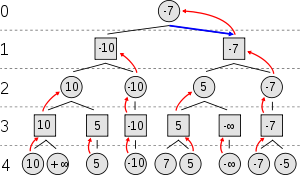
\includegraphics[width=300pt]{minimax_example}
	\label{fig:minimax_example}
\end{figure}

Мінімаксний алгоритм потребує функцію генерування можливих ходів (ходи, що не є заборонені правилами гри) та функцію еврістичної оцінки поточного стану дошки. Розробка функції оцінки стану виходить за рамки даної роботи, тому замість неї буде використовуватися випадкова величина.

Функція генерування можливих ходів (movegen у коді) використовує поточний стан дошки board та колір гравця, що робить крок player. Гравець завжди комп'ютер, але функції потрібно знати його колір, щоб вирішувати куда можно ставити камінь, адже всередину груп з однією ступінню свободи може ходити тільки гравець, чия ця група. Функція повертає список можливих ходів у вигляді пар координат. Саме ця функція має найбільші знання про гру Го. Вона повинна розуміти правило зняття з дошки каменів та правило Ко.

Алгоритм Мінімакс можно досить легко розпаралелити. Достатньо шукати максимум кожного піддерева у окремому потоці. В мові Clojure це можна легко зробити використовуючи функцію pmap. Ця функція працює як звичайний map, але запускає функції у окремих потоках, повертаючи Future. Використовуючи цей об'єкт можливо дізнатися коли закінчиться виконання відповідної функції та отримати її результат.

Така функція дозволяє досить просто розпаралелити функцію Мінімаксу, але віна не дає змогу контролювати цей процес. Якщо є така задача, то розпаралелення можна реалізувати самостійно, використовуючи ті самі об'єкти типу Future.

\begin{algorithmic}
	\Function{minimax}{node, depth}
	\Comment returns integer - value of best play
		\If {node is a terminal node \textbf{or} depth $\leq$ 0}
			\State \Return the heuristic value of node
		\EndIf
	    \State $\alpha\gets-\infty$
		\For {child \textbf{in} node}
			\Comment evaluation is identical for both players
			\State $\alpha\gets$max($\alpha$, -minimax(child, depth-1))
		\EndFor
		\State \Return $\alpha$
	\EndFunction
\end{algorithmic}

\subsection{Альфа-бета відсічення}
Альфа-бета відсічення —- алгоритм пошуку, що зменшує кількість вузлів, які необхідно оцінити в дереві пошуку мінімаксного алгоритму і при цьому дозволяє отримати ідентичний результат. Цей алгоритм використовується в програмуванні ігор, де грають два гравці (хрестики-нулики, шахи, го). Використовуючи цей алгоритм, програма повністю припиняє оцінювати хід, якщо знайшла доказ, що цей хід гарантовано гірший, ніж оцінений раніше. Такі ходи не потребують подальшого розглядання.

\begin{figure}[H]
	\centering
	\caption{Ілюстрація роботи алгоритму Альфа-бета відсічення}
	\includegraphics[width=300pt]{AB_pruning}
	\label{fig:AB_pruning}
\end{figure}

Альфа-бета алгоритм, при найкращому порядку ходів, побудує значно менше дерево перебору. Кількість вузлів приблизно дорівнює кореню квадратному з числа позицій, що переглядаються при повному переборі. Альфа-бета розподіл дуже чутливий до порядку ходів. Тому потрібно врахувати, що при найгіршому порядку ходів, тобто коли відсічення за beta розглядає останній хід, альфа-бета алгоритм прогляне стільки ж позицій, що і мінімакс. Швидкість прорахунку також дуже залежить на практиці від можливого діапазону оцінок.

Приклад псевдокоду Альфа-бета відсічення:

\begin{algorithmic}
	\Function{AlphaBeta}{color, depth, $\alpha$, $\beta$}
		\If {depth = 0}
			\State \Return \Call{Evaluate}{color}
		\EndIf
		\State moves $\gets$ \Call{GenerateMoves}{}
		\For {move \textbf{in} moves}
			\State \Call{makeMove}{move}
			\State eval $\gets$ -\Call{AlphaBeta}{-color, depth-1, -$\beta$, -$\alpha$}
			\State \Call{unmakeMove}{move}
			\If {eval $\geq \beta$}
				\State \Return $\beta$
			\EndIf
			\If {eval $> \alpha$}
				\State $\alpha \gets$ eval
				\If {depth = defaultDepth}
					\State bestmove $\gets$ move
				\EndIf
			\EndIf
		\EndFor
		\State \Return $\alpha$
	\EndFunction
\end{algorithmic}

\subsection{Порівняння з шаблоном}
Єфективне роспізнання шаблонів у грі Го та їх грамотне використання є вирішальним як для гравця-людини, так і для програми. На поточний момент було створено базу шаблонів різних етапів партії на основі професійних партій в Го. Така база використовуються майже усіма програмами, що грають у Го.

Не зважаючи на те, що велику кількість шаблонів партій з Го можна знайти в спеціалізованих базах даних, краще ці шаблони та статистику їх використання з'ясувати самим.

Спочатку дамо визначення шаблону партії Го. Шаблоном будемо називати послідовність ходів у партії, що обмежені квадратом 5x5 з першим ходом у центрі. Такий підхід дозволить швидко знаходити нові шаблони, до того ж аналізувати статистику їх використання.

\begin{figure}[H]
	\centering
	\caption{Приклад першого ходу у шаблонах в грі го}
	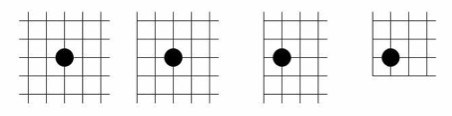
\includegraphics[width=300pt]{go_pattern_example}
	\label{fig:go_pattern_example}
\end{figure}

Також необхідно розробити метод, який би об'єднував однакові шаблони у один, з урахуванням повороту, симетрії та зміні кольору каменів на протилежний. Один із методів, що можна використати, заснований на канонічній формі шаблона.

Щоб привести шаблон до канонічної форми спочатку інвертуємо кольори ходів, якщо потрібно, щоб перший хід був чорним. Далі всього 8 варіантів перетворень можливо (4 повороти $\times$ 2 симетрії). Закодуємо кожен з цих варіантів одним числом Integer (наприклад, використовуючи Зобріст-хешування, що буде описано далі). Канонічною формою шаблону будемо називати варіант, що має найменше відповідне закодоване значення. Таким чином можливо 4 варіанти, що відображені на рис. \ref{fig:go_canonical_pattern} звести до одного.

\begin{figure}[H]
	\centering
	\caption{Приклад однакових шаблони, що повинні об'єднатися в один}
	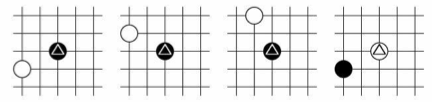
\includegraphics[width=300pt]{go_canonical_pattern}
	\label{fig:go_canonical_pattern}
\end{figure}

Далі треба створити базу шаблонів з статистичними даними, по цих зразках. Найпростіше збирати інформацію про кількість разів, яку цей шаблон був використаний у партіях, що були проаналізовані. Якщо використовувати велику кількість партій професійного рівня, то така статистика може використовуватися програмами, що грають в го, як база даних гарних ходів. Вони можут шукати частини шаблонів у іграх, а потім догравати використовуючи ті варіанти, що більш вигідні їм.

Наведемо приклад алгоритму створення подібної бази шаблонів з колекції ігор:

\begin{algorithmic}
	\For {each game record R \textbf{in} the game record collection}
		 \For {each move M \textbf{in} R}
		 	\State Play M on the game board
			\State Obtain the 5-by-5 region R centered by M
			\State Rotate and flip R into its canonical form
			\If {R is \textbf{not in} our pattern database}
				\State Add R into the pattern database
				\State Set frequency number of R to be 0
			\EndIf
			\State Increase the frequency number of R by 1
		\EndFor
	\EndFor
\end{algorithmic}

Завдяки аддитивності Зобріст-хешування пошук шаблону по такій базі дуже простий. Якщо не враховувати можливі колізії, то перевірка наявності шаблону (тобто підпослідовності ходів) у партії зводиться до виконанню операції XOR над хешом шаблону та хешом поточного стану партії. Це є дуже ефективним способом знаходення шаблонів, однак недолік полягає у тому, що таку перевірку треба робити для всіх станів дошки партії починаючи з якогось. Тобто для знаходження шаблонів у партії в 200 ходів, використовуючи базу даних з 1000 шаблонів треба виконати 200 тисяч операцій XOR.

\subsection{Зобріст хешування}
Одним із методів пошуку деякого положення каменів на дошці може будти хешування. Якщо використовувати хешування, по якому можна легко дізнатися, що стоїть на якій клітинці, то функція пошуку деякого зразка на дошці теж буде досить легкою. Прикладом такого хешування может бути Зобріст-хешування.

Зобріст-хешування -- це хеш-функція, що використовується в комп'ютерних програмах, які грають  в абстрактні настільні ігри, такі як шахи або го і використовують транспозиційні таблиці, особливий вид хеш-таблиць, що індексуються позиціями дошки і використовується, щоб уникнути аналізу однієї і тієї ж самої позиції декілька разів.

Зобріст-хешування починається з генерування випадкового бітового рядка для кожного можливого елемента настільної гри, тобто для кожної комбінації фігури і положенням (у грі в шахи, це 12 штук $\times$ 64 позицій дошки, для го, це 2 фігури $\times$ 361 позицій дошки). Тепер будь-якоа конфігурація дошки може бути розбита на незалежні компоненти фігура/положення, кожен з яких має відповідний бітовий рядок. Остаточний Зобріст хеш обчислюється через ці бітові рядки використовуючи побітовое XOR між усіма ними.

Приклад псевдокоду для гри в Го:

\begin{algorithmic}
	\State empty $\gets$ 0
	\Comment{constant figures}
	\State white\_stone $\gets$ 1
	\State black\_stone $\gets$ 2
	\Function{init\_zobrist}{}
	\Comment{fill a table of random numbers/bitstrings}
		\State table $\gets$ a 2-d array of size 361$\times$2
		\For{i \textbf{from} 1 \textbf{to} 361}
		\Comment{loop over the board, as a linear array}
			\For{j \textbf{from} 1 \textbf{to} 2}
			\Comment{loop over the figures}
				\State table[i][j] $\gets$ \Call{random\_bitstring}{}
			\EndFor
		\EndFor
	\EndFunction
	\Function{hash}{board}
		\State h $\gets$ 0
		\For{i \textbf{from} 1 \textbf{to} 361}
		\Comment{loop over the board positions}
			\If{board[i] $\neq$ empty}
				\State j $\gets$ the piece at board[i], as listed in the constant figures, above
				\State h $\gets$ h XOR table[i][j]
			\EndIf
		\EndFor
		\State \Return h
	\EndFunction
\end{algorithmic}

\subsection{Метод Монте-Карло}
Метод Монте-Карло -- загальна назва групи числових методів, основаних на одержанні великої кількості реалізацій стохастичного (випадкового) процесу, який формується у той спосіб, щоб його ймовірнісні характеристики збігалися з аналогічними величинами задачі, яку потрібно розв'язати. Використовується для розв'язування задач у фізиці, математиці, економіці, оптимізації, теорії управління тощо.

Метод Монте-Карло — це метод імітації для приблизного відтворення реальних явищ. Він об'єднує аналіз чутливості (сприйнятливості) і аналіз розподілу ймовірностей вхідних змінних. Цей метод дає змогу побудувати модель, мінімізуючи дані, а також максимізувати значення даних, які використовуються в моделі. Побудова моделі починається з визначення функціональних залежностей у реальній системі. Після чого можна одержати кількісний розв'язок, використовуючи теорію ймовірності й таблиці випадкових чисел.

Для пошуку гри в Го існує метод Монте-Карло пошуку по деревах. Він генерує велику кількість випадкових партій до кінця гри. Потім він рахує статистику виграшу та програшу у цих іграх. Використовуючи цю статистику, він приймає рішення щодо наступного ходу, вибираючи хід, що має найбільшу вірогідність виграшу.

Цей метод потребує розширення структури дерева варіантів гри. Він додає 2 значення у кожний вузол: статистику виграшів ($winrate \in [0; 1]$) та число раз, що цей вузол був відвіданий. На основі цих двох значень використовуючи функцію, показану нижче, алгоритм вираховує найкращий шлях для продовження аналізу на початку кожного кроку.

\begin{equation*}
    UCTValue(parent,n)=winrate+\sqrt{\frac{\ln(parent.visits)}{5\times n.nodevisits}}
\end{equation*}

Алгоритм має таку структуру:
\begin{itemize}
	\item Вибір найкращого можливого маршруту
	\item Продовження кінцевого вузла випадковим чином
	\item Симуляція великої кількості випадкових ігор
	\item Оновлення значень в усіх пройдених вузлах
	\item Повторення з початку
\end{itemize}

\subsection{Обробка SGF-файлів}
Smart Game Format (SGF) -- комп'ютерний формат даних, що зберігає партії ігор, таких як Го, шахи, шашки та реверсі. Це простий, текстовий формат, що зберігає партії у вигляді дерев.

Були розроблені функції, що дозволяють маніпулювати цим файлом: читати його, перетворювати у внутрішній формат, спрощувати дерево, перетворювати у формат, що відображає положення дошки, та вивід цієї дошки на монітор.

Читання та перетворення SGF-файлу запрограмовано у вигляді лексеру та парсеру. Лексер має на вході послідовність символів з файлу, що читаються по мірі необхідності, а генерує послідовність лексем. Тобто ключових слів, що притаманні данному формату.

Список реалізованих лексем:
\begin{itemize}
	\item :treestart
	\item :treeend
	\item :nodestart
	\item :propvalue
	\item :propvalueend
	\item :propident
\end{itemize}

Далі використовується функція, що парсить список лексем, генеруючи дерева властивостей. Саме ця функція повинна знати граматичні правила даного формату.

Найчастіше для пошуку потрібні тільки ті властивості у дереві гри, що відповідають позиціям каменів гравців, усі ж інші властивості -- зайві. Тому була реалізована функція simplify, що фільтрує та спрощує дерево гри, залішаючи тільки послідовність ходів гравців. З такою структурою даних набагато легше працювати, до того ж вона займає менше пам'яті комп'ютера.

Досить часто доцільніше використовувати іншу структуру даних, що репрезентує поточний стан дошки. Ця структура вже не дерево, вона має вигляд матриці значень клітинок дошки (тобто ця клітинка пуста, зайнята білим каменем, або зайнята чорним каменем). Ця структура більш зручна, якщо треба аналізувати поточний стан дошки, адже дерево не має у собі таку інформацію. Ця структура даних необхідна для методу пошуку шаблону, саме на її основі рахується хеш поточного стану дошки.

Для візуалізації поточного стану дошки використовується функція print-board, що виводить на монітор дошку з каменями гравців. Вивід цієї функції схожий на вивід дошки у програмі GnuGo.

\begin{figure}[H]
	\centering
	\caption{Приклад виводу функції print-board}
	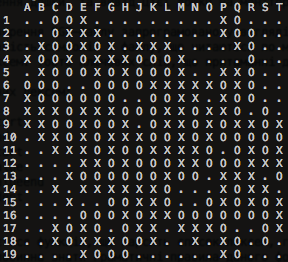
\includegraphics[width=230pt]{print-board}
	\label{fig:print-board}
\end{figure}


	% \newpage
\section{Аналіз розроблених програмних засобів}
\subsection{Методика тестування програмного засобу}
\subsection{Аналіз швидкодії алгоритмів та якості пошуку}


	% \newpage
\section{OХОРОНА ПРАЦІ}
Дана дипломна робота передбачає розробку програмного засобу для пошуку у структурах даних гри Го.  Розробка даної програми відбувається в кімнаті офісу на чотирьох осіб, у кожної з яких є робоче місце на один комп’ютер.

Правильно організована робота по забезпеченню безпеки праці підвищує дисциплінованість працівників, поліпшує умови праці, що в свою чергу, призводить до підвищення продуктивності праці, зниження кількості нещасних випадків, запобігання  виходу з ладу обладнання та інших нештатних ситуацій.

Покращення умов праці та її безпека призводить до зменшення виробничого травматизму, професійних хвороб, що зберігає здоров’я працівників та одночасно призводить до зменшення затрат на оплату пільг та компенсацій, на оплату наслідків такої роботи, на лікування, перепідготовку працівників виробництва в зв’язку зі зміною кадрів через причини, що пов’язані з умовами праці.
\subsection{Аналіз робочого місця}
Приміщення, в якому розроблювалася система буде розташоване на другому поверсі п'ятиповерхового будинку та розраховано на чотири робочих місця. Схема приміщення представлена нижче:

\begin{figure}[H]
	\centering
	\caption{Схематичний план приміщення}
	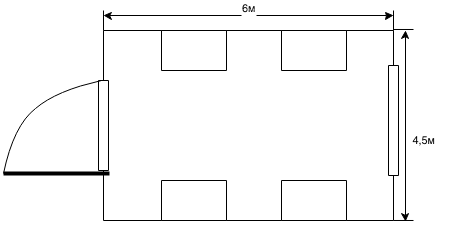
\includegraphics[width=150pt]{safety_room_plan}
	\label{fig:safety_room_plan}
\end{figure}

\begin{tabular}{l}
	Довжина приміщення: 6м;\\
	Ширина приміщення: 4.5м;\\
	Висота приміщення: 3.5м;\\
	Колір підлоги – темний, стін та стелі – світлий.\\
	Коефіцієнти відображення:
\end{tabular}

\begin{equation}
	\rho_\textup{стелі}=70\%,
	\rho_\textup{стін}=50\%,
	\rho_\textup{підлоги}=30\%
\end{equation}

\begin{tabular}{l}
	В приміщенні є одне вікно розмірами: 1.5 м шириною і 2 м висотою.\\
	Площа даного приміщення: $S=6\textup{м}*4.5\textup{м}=27\textup{м}^2$ \\
	Об'єм даного приміщення: $V=S*h=27\textup{м}^2*3.5\textup{м}=94.5\textup{м}^3$\\
	Таким чином, на одне робоче місце надано: $S=6.75\textup{м}^2, V=23.625\textup{м}^3$\\
	Порівняємо розрахункові значення з нормативними у таблиці:
\end{tabular}

\begin{table}[H]
	\centering
	\caption{Розрахункові та нормативні значення площі та об'єму приміщення з розрахунку на одне рабоче місце}
	\begin{tabular}{| l | l | l |}
		\hline
		Параметр приміщення & Нормативний & Розрахунковий\\\hline
		Площа, $\textup{м}^2$ & 6 і більше & 6.75\\\hline
		Об'єм, $\textup{м}^3$ & 20 і більше & 23.625\\\hline
	\end{tabular}
\end{table}

Отже, можна зробити висновок, що площа та об’єм робочого місця відповідає нормам НПАОП 00.0-1.28-10.
\subsection{Аналіз шкідливих і небезпечних факторів}
\subsubsection{Мікроклімат}
Санітарні норми мікроклімату виробничих приміщень в цьому розділі описані згідно ДСН 3.3.6.042-99. Робота, виконувана в даному приміщенні відноситься до категорії робіт – «Легка 1б». У приміщеннях з використанням обчислювальної техніки рекомендується застосування тільки оптимальних значень показників мікроклімату. Нижче приведено видповідні санітарні вимоги до мікроклімату в приміщенні, що повинні дотримуватися.

\begin{table}[H]
	\centering
	\caption{Оптимальні значення параметрів мікроклімату для категорії робіт ``Легка-1б''}
	\begin{tabular}{| l | r | r | r | }
		\hline
		Пора року & Температура, $^oC$ & Вологість, \% & Швидкість повітря, м/с \\\hline
		Тепла & 22-24 & 40-60 & 0,1 \\\hline
		Холодна	& 21-23 & 40-60 & 0,1 \\\hline
	\end{tabular}
	\label{tab:micro-climate}
\end{table}

У приміщенні встановлені батареї центрального водяного опалення, що включається в холодний період року. У теплу пору працює, система кондиціонування, що складається з кондиціонера спліт-системи Кондиціонер DELFA ADW-07C з потужністю 1100 Вт.
\subsubsection{Освітлення}
В приміщеннях для роботи з ЕОМ повинне використовуватися як природне так і штучне освітлення. Природне освітлення забезпечує вікно, загальна площа якого складає $3\textup{м}^2$. Воно являється боковим та одностороннім.

Нормоване значення КПО, яке має забезпечувати природне освітлення розраховується за формулою:

\begin{equation}
	e_\textup{н}=\frac{S_\textup{вік}}{S_n}=\frac{3}{27}=0.11,
\end{equation}
 
де $e_\textup{н}$ -- значення КПО; $S_\textup{вік}$ -- загальна площа вікна, $\textup{м}^2$; $S_n$ -- площа підлоги, $\textup{м}^2$. 

Отримане значення $0.11$ менше ніж встановлено нормами (КПО має бути не меншим за $0.15$), тобто природного освітлення не вистачає для нормальної роботи. Тому потрибно використовувати штучне освітлення.

Штучне освітлення в приміщеннях з робочими місцями, обладнаними ВДТ ЕОМ та ПЕОМ, має здійснюватися системою загального рівномірного освітлення. У якості джерел світла для штучного освітлення мають застосовуватись переважно люмінесцентні лампи типу ЛБ, потужністю 20Вт. Для загального освітлення слід застосовувати 2 світильники серії ЛПО, розташовані у 2 ряди. Один світильник містить 2 лампи, кожна з яких має світловий потік 1060 лм. Нормативна освітленість 300-400 лк., згідно ДБН 2006. Штучне освітлення кімнати створює освітленість 340 лк, що задовольняє стандарту.
\subsubsection{Шум}
Основним джерелом шуму є системний блок комп’ютера, який містить такі компоненти як: жорсткий диск та кулер.

Таким чином у приміщенні мають місце шуми механічного і аеродинамічного походження. Шум, що створюється, умовно можна віднести до постійного.

Згідно з ДСН 3.3.6.037-99 допустимий шум на постійних робочих місцях користувача складає до 50 дБА. Орієнтовні еквівалентні рівні звукового тиску джерел шуму, що діють на користувача на його робочому місці, представлені в табл. \ref{tab:sound_levels}.

\begin{table}[H]
	\centering
	\caption{Рівні звукового тиску від різних джерел}
	\begin{tabular}{| l | r | }
		\hline
		Джерело шуму & Рівень шуму, дБА \\\hline
		Жорсткий диск & 26 \\\hline
		Кулер & 28 \\\hline
	\end{tabular}
	\label{tab:sound_levels}
\end{table}

Розрахуємо середній рівень шуму на робочому місці користувача при роботі всієї вказаної техніки.

Рівень шуму, що виникає від декількох некогерентних джерел, що працюють одночасно, підраховується на підставі принципу енергетичного підсумовування рівня інтенсивності окремих джерел:

\begin{equation}
	L = 10\lg\sum10^{0.1L_i},
\end{equation}
де $L_i$ -- рівень звукового тиску і-того джерела.

Підставивши значення рівня звукового тиску для кожного виду устаткування у формулу, отримаємо: 

\begin{equation}
	L = 10\lg(4*10^{0.1*26}+4*10^{0.1*28})=36\textup{дБ}.
\end{equation}

Розраховане значення рівня шуму не перевищує гранично допустимого рівня шуму для робочого місця користувача (50 дБА), тобто спеціальні заходи по зниженню рівня шуму не потрібні.

Таким чином, робота з системою, розробленою в дипломній роботі, являється безпечною і не потребує додаткових улаштувань для зниження шуму, окрім загальних методів ізоляції від зовнішнього шуму. Для цього застосовуються  спеціальні віконні профілі та звукоізоляція зовнішніх стін плитами зі звукоізоляційними наповнювачами.
\subsection{Електромагнітні випромінювання}
Більшість учених вважає, що як короткочасна, так і тривала дія всіх видів випромінювання від екрану монітора не небезпечна для здоров'я людини. Проте вичерпних даних щодо небезпеки дії випромінювання від моніторів на людей, що працюють з комп'ютерами не існує і дослідження в цьому напрямі продовжуються.

Допустимі значення параметрів не іонізуючих електромагнітних випромінювань від монітора комп'ютера представлені в табл. \ref{tab:x-ray}.

Максимальний рівень рентгенівського випромінювання на робочому місці оператора комп'ютера звичайно не перевищує 10мкбэр/ч, а інтенсивність ультрафіолетового і інфрачервоного випромінювань від екрану монітора лежить в межах 10-100мВт/м$^2$.

\begin{table}[H]
	\centering
	\caption{Допустимі значення параметрів не іонізуючих електромагнітних випромінювань}
	\begin{tabular}{| l | r | }
		\hline
		Найменування параметра & Допустимі \\\hline
	    Напруженість електричної складової електромагнітного & \\
		поля на відстані 50см від поверхні відеомонітора & 10В/м \\\hline
	    Напруженість магнітної складової електромагнітного & \\
		поля на відстані 50см від поверхні відеомонітора & 0.3А/м \\\hline
		Напруженість поля не повинна перевищувати:  & \\
		для дорослих користувачів & 20кВ/м \\
		для дітей дошкільних установ і що вчаться в & 15кВ/м \\
		середніх спеціальних і вищих учбових закладів & \\\hline
	\end{tabular}
	\label{tab:x-ray}
\end{table}

Для зниження дії цих видів випромінювання рекомендується застосовувати монітори із зниженим рівнем випромінювання (MPR-II, TCO-92, TCO-99, TCO-03), а також дотримувати регламентовані режими праці і відпочинку.
\subsection{Електробезпека}
Згідно з ДНАОП 0.00-1.3.1-99 робоче місце підпадає під категорію без підвищеної небезпеки.

Електроустаткування належить до приладів до 1000 В. Устаткування, що використовується, відповідно до ПУЄ належить до устаткування класів 0, 0І, і І за електрозахистом.

Оцінка небезпеки дотику до струмових частин відноситься до визначення сили струму, що протікає через тіло людини, і порівняння його із допустимим значенням відповідно до ГОСТ 12.1.038-88.

Лінія електромережі для живлення персональних комп'ютерів, їх периферійних пристроїв (принтер) виконується як окрема групова три-провідна мережа, шляхом прокладання фазового, нульового робочого та нульового захисного провідників. Нульовий захисний провідник використовується для заземлення електроприладів. Провід мідний, ізоляція має бути закритою, марки ПУНП, перерізом не менше 2,5х2мм на жилу. Частота струму не має перевищувати значення 50 Гц.

При виконанні розрахунків для дипломного проекту використовувався персональний комп'ютер - І і II клас захисту, що живиться напругою 220 В. Для правильного визначення необхідних засобів та заходів захисту від ураження електричним струмом необхідно знати допустимі значення напруг доторкання та струмів, що проходять через тіло людини.

Гранично допустимі значення напруги доторкання та сили струму для нормального (безаварійного) та аварійного режимів електроустановок при проходженні струму через тіло людини по шляху ``рука – рука'' чи ``рука – ноги'' регламентуються ГОСТ 12.1.038-88 (табл. \ref{tab:current}).

\begin{table}[H]
	\centering
	\caption{Граничнодопустимі значення напруги доторкання та сили струму, що проходить через тіло людини при нормальному режимі електроустановки}
	\begin{tabular}{| l | r | r |}
		\hline
		Вид струму & В (не більше) & мА (не більше) \\\hline
		Змінний, 50Гц & 2 & 0.3 \\\hline
		Змінний, 400Гц & 3 & 0.4 \\\hline
		Постійний & 8 & 1.0 \\\hline
	\end{tabular}
	\label{tab:current}
\end{table}
\subsection{Пожежна безпека}
Згідно з НАПБ Б.03.002-2007 таке приміщення відноситься до категорії    В–пожежонебезпечна. При нормальному режимі роботи можливість виникнення пожежі мінімальна. Можливість виникнення вибухів повністю відсутня. Можливими причинами загоряння можуть бути пошкодження та замикання в електромережі та електрообладнанні, а також порушення правил безпеки при роботі з обладнанням.

На робочому місці наявні наступні пожежонебезпеці матеріали: папір, пластик, віконні рами, дерев’яні шафи, корпуси техніки, меблі. Робоче приміщення повинно бути обладнане двома вуглекислотними вогнегасниками ВВК-5 з розрахунку два вогнегасника на приміщення  до   25 кв.м  включно, що задовольняє НАПБ Б.03.002-2007. Для захисту від блискавки будівля обладнана блискавковідводом стрижневого типу.

В приміщенні посередині стелі має бути встановлений один димовий пожежний сповіщувач СПД-3 відповідно до ДБН В.1.1.-7-2002 – з розрахунку один на висоту до 3,5 м та загальною площею не більше ніж 86 м$^2$.

Технічні заходи щодо зниження пожежної небезпеки на підприємстві:
\begin{itemize}
	\item застосування засобів пожежогасіння;
	\item використання засобів пожежної сигналізації;
	\item проведення пожежотехнічних обстежень;
	\item використання знаків.
\end{itemize}

    \conclusion

    Деякі висновки.

    \begin{thebibliography}
\bibitem{Landafshitz}
Ландау~Л.~Д., Лившиц~Е.~М. Теоретическая физика: Учеб. пособ.: Для вузов. В 10 т. Т. VI. Гидродинамика. --- 5-е изд., стереот. --- М.:~ФИЗМАТЛИТ. --- 2001. --- 736~с. --- ISBN5-9221-0121-8 (T. VI).

\bibitem{Sokolofsky}
Sokolofsky~S.~A., Jirka~J.~A. CVEN 489-501: Special Topics on Mixing and Transport in the Environment. Engineering -- Lectures. --- 5th edition. --- Texas A \& M University. --- 2005. --- 184~pp.

\bibitem{Bejan}
Adrian~Bejan. Convection Heat Transfer. --- 4th edition. --- Wiley. --- 2013. --- 696~pp.

\bibitem{Lewis}
Lewis~R.~W. Fundamentals of the Finite Element Method for Heat and Fluid Flow. / Ronald~W.~Lewis, Perumal Nithiarasu, Kankanhally N. Seetharamu. --- Wiley. --- 2004. --- 356~pp.

\bibitem{Vlasova}
Власова~Е.~А. Приближенные методы математической физики. / Е.~А.~Власова, В.~С.~Зарубин, Г.~Н.~Кувырикин. --- М.:~Изд-во МГТУ им.~Н.~Э.~Баумана. --- 2001. --- 700~с.

\bibitem{Brebbia}
Бреббия~К. Метод граничных элементов: Пер. с англ. / Бреббия~К., Теллес~Ж., Вроубел~Л. --- М.:~Мир. --- 1987. --- 524~с.

\end{thebibliography}


\end{document}
